\section{Risultati}
Per confrontare gli attacchi è stato eseguito $run\_benchmark$ sulla suite $regular$.
Questa suite è composta da 4 gruppi di percorsi basati sulle mappe NoCrashTown01 e NoCrashTown02. Ogni gruppo fornisce un percorso ripetuto tre volte con diverse condizioni meteorologiche.
Un percorso viene considerato non completato se avviene una collisione oppure se il veicolo non arriva al goal entro il limite di tempo (timeout).

Il percorso in NoCrashTown01 prevede una singola curva a destra, mentre in NoCrashTown02 sono presenti svolte e incroci multipli.
I 4 gruppi hanno le seguenti caratteristiche:\begin{itemize}
    \item NoCrashTown01-v3\begin{itemize}
        \item condizioni metereologiche: ClearNoon (mezzogiorno, nuvoloso con asfalto asciutto), WetNoon (mezzogiorno, nuvoloso con asfalto bagnato) e HardRain (mezzogiorno, pioggia intensa con asfalto bagnato);
        \item numero di veicoli:20;
        \item numero di pedoni:50.
    \end{itemize}
    \item NoCrashTown02-v3 \begin{itemize}
        \item condizioni metereologiche: ClearNoon, WetNoon e HardRain;
        \item numero di veicoli:15;
        \item numero di pedoni:50.
    \end{itemize}
    \item NoCrashTown01-v4 \begin{itemize}
        \item condizioni metereologiche: WetSunset (tramonto, sereno con asfalto bagnato) e SoftRainSunset (tramonto, pioggia debole  con asfalto bagnato). WetSunset è usato in due percorsi;
        \item numero di veicoli:20;
        \item numero di pedoni:50.
    \end{itemize}
    \item NoCrashTown02-v4 \begin{itemize}
        \item condizioni metereologiche: WetSunset  e SoftRainSunset;
        \item numero di veicoli:15;
        \item numero di pedoni:50.
    \end{itemize}
\end{itemize}

La valutazione degli attacchi si è svolta in due fasi:\begin{itemize}
    \item nella prima, i percorsi sono stati seguiti da un agente senza nessun attacco iniettato (golden run);
    \item nella seconda fase, si eseguono le stesse run della prima, ma ogni volta con un diverso attacco iniettato.
\end{itemize}
I risultati prodotti dall'iniezione di ciascun attacco sono stati confrontati con quelli prodotti dalla golden run, in modo da valutarne l'efficacia.
Il confronto è stato fatto con l'analisi dei video prodotti (disponibili a \href{https://drive.google.com/drive/folders/1tTEAQSK2XAK_sdmuWo80Bd-58_pkiK3h?usp=sharing}{\emph{questo indirizzo}}), valutando i percorsi portati a termine,  la stabilità della guida, i semafori rossi ignorati e le cause dei percorsi
non completati (collisioni e timeout).
\subsection{Golden Run}
\begin{table}[h]
    \begin{tabular}{|c|c|c|}
        \hline
        Mappa                   & Run completate & Percentuale di completamento\\
        \hline
        NoCrashTown01-v3        & 3/3            & 100\% \\
        NoCrashTown01-v4        & 3/3            & 100\% \\
        NoCrashTown02-v3        & 3/3            & 100\% \\
        NoCrashTown02-v4        & 3/3            & 100\%  \\
        \hline
        \textbf{TOTALE}                  & 12/12          & 100\% \\
        \hline
    \end{tabular}
    \caption{Risultati golden run.}
Nella golden run tutti i percorsi vengono completati con successo. La traiettoria del veicolo è stabile, nessun semaforo è stato ignorato e non si sono registrate collisioni.
\end{table}
\begin{figure}[h!]
    \centering
    \parbox{6cm}{
    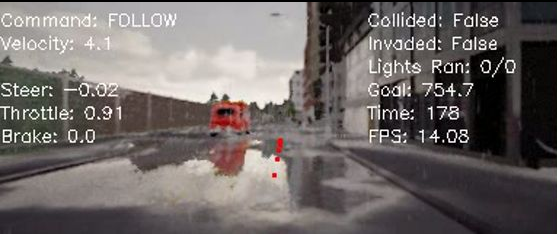
\includegraphics[width=6cm]{GOLD1.png}
    \label{fig:gold1}}
    \qquad
    \begin{minipage}{6cm}
    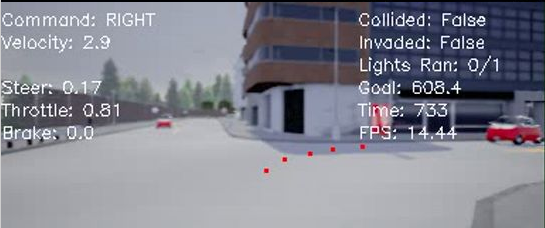
\includegraphics[width=6cm]{GOLD2.png}
    \label{fig:gold2}
    \end{minipage}
    \caption{Golden run.}
    \label{fig:goldrun}
    \end{figure}
\newpage
\subsection{Iniezione di HopSkipJump (HSJ)}
\begin{table}[h]
    \begin{tabular}{|c|c|c|}
        \hline
        Mappa                   & Run completate & Percentuale di completamento\\
        \hline
        NoCrashTown01-v3        & 3/3            & 100\% \\
        NoCrashTown01-v4        & 2/3            & 66\% \\
        NoCrashTown02-v3        & 1/3            & 33\% \\
        NoCrashTown02-v4        & 0/3            & 0\%  \\
        \hline
        \textbf{TOTALE}                  & 6/12           & 50\% \\
        \hline
    \end{tabular}
    \caption{Risultati run HopSkipJump}
    \label{tab:hsj}
\end{table}
La macchina continua a seguire il percorso prestabilito in modo molto più instabile. L'instabilità è particolarmente evidente negli waypoints generati, che cambiano continuamente posizione anche nei rettilinei. A causa dei problemi elencati
si nota un aumento dei semafori ignorati (9) e delle uscite fuori strada. I fallimenti (6) sono stati tutti causati da collisioni.
\begin{figure}[h]
    \centering
    \parbox{6cm}{
    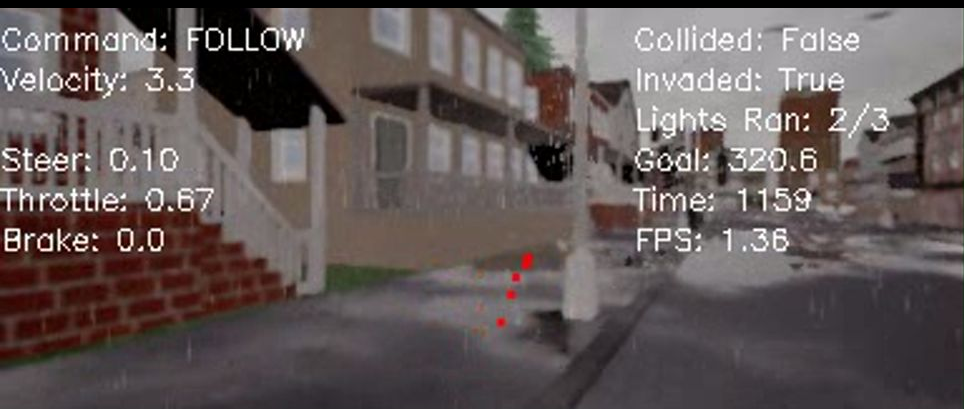
\includegraphics[width=6cm]{hoprun.png}
    \label{fig:hop1}}
    \qquad
    \begin{minipage}{6cm}
    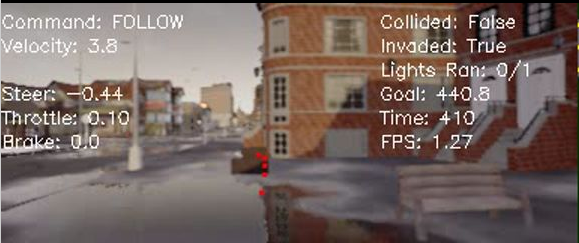
\includegraphics[width=6cm]{HOP2.png}
    \label{fig:hop2}
    \end{minipage}
    \caption{Collisioni causate da HopSkipJump.}
    \label{fig:hoprun}
    \end{figure}
\newpage
\subsection{Iniezione di Spatial Transformation (STA)}
\begin{table}[h!]
    \begin{tabular}{|c|c|c|}
        \hline
        Mappa                   & Run completate & Percentuale di completamento\\
        \hline
        NoCrashTown01-v3        & 2/3            & 66\% \\
        NoCrashTown01-v4        & 3/3            & 100\% \\
        NoCrashTown02-v3        & 1/3            & 33\% \\
        NoCrashTown02-v4        & 1/3            & 33\%  \\
        \hline
        \textbf{TOTALE}                  & 7/12           & 0\% \\
        \hline
    \end{tabular}
    \caption{Risultati run Spatial Transformation.}
    \label{tab:sta}
\end{table}
Nelle run completate la macchina si comporta normalmente. Non si notano variazioni rilevanti nella traiettoria e nessun semaforo viene ignorato. Delle 5 run
non completate, quattro sono terminate per collisione avvenuta e una per timeout. In queste run si nota una tendenza del veicolo ad andare largo alle curve, fino ad invadere la corsia opposta e causare un incidente.
In una run la macchina esce subito di strada andando a sbattere contro un edificio nelle vicinanze.
\begin{figure}[h]
    \centering
    \parbox{6cm}{
    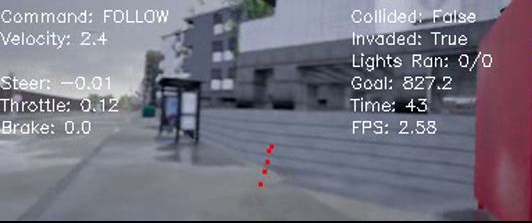
\includegraphics[width=6cm]{STA1.png}
    \label{fig:sta1}}
    \qquad
    \begin{minipage}{6cm}
    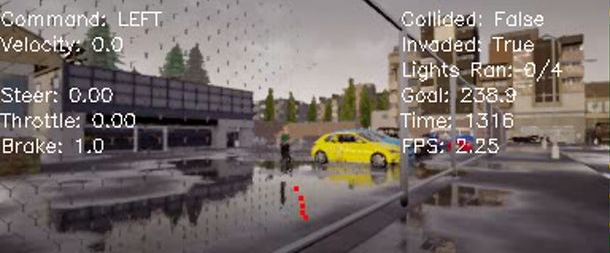
\includegraphics[width=6cm]{STA2.png}
    \label{fig:sta2}
    \end{minipage}
    \caption{collisioni causate da Spatial Transformation}
    \label{fig:starun}
    \end{figure}
\subsection{Iniezione di Basic Iterative Method (BIM)}
\begin{table}[h]
    \begin{tabular}{|c|c|c|}
        \hline
        Mappa                   & Run completate & Percentuale di completamento\\
        \hline
        NoCrashTown01-v3        & 0/3            & 0\% \\
        NoCrashTown01-v4        & 0/3            & 0\% \\
        NoCrashTown02-v3        & 0/3            & 0\% \\
        NoCrashTown02-v4        & 0/3            & 0\%  \\
        \hline
        \textbf{TOTALE}                  & 0/12           & 0\% \\
        \hline
    \end{tabular}
    \caption{Risultati run Basic Iterative Method.}
    \label{tab:bim}
\end{table}
La guida autonoma risulta compromessa. In nessuno dei percorsi la macchina segue il tragitto, ma invece sterza subito verso destra fino ad uscire di strada
e urtare oggetti della mappa.
\begin{figure}[h]
    \centering
    \parbox{5cm}{
    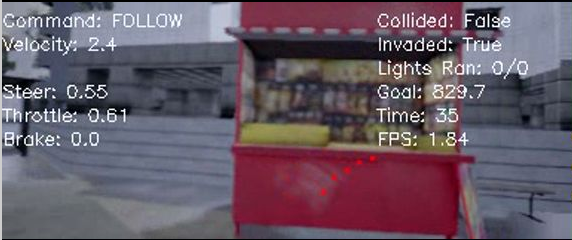
\includegraphics[width=5cm]{BIM1.png}
    \label{fig:bim1}}
    \qquad
    \begin{minipage}{5cm}
    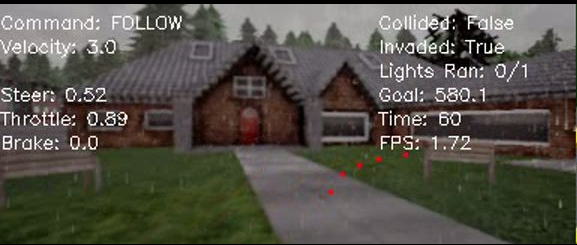
\includegraphics[width=5cm]{BIM2.png}
    \label{fig:bim2}
    \end{minipage}
    \caption{Collisioni causate da Basic Iterative Method.}
    \label{fig:bimrun}
    \end{figure}
\newpage
\subsection{Iniezione di NewtonFool (NF)}
\begin{table}[h!]
    \begin{tabular}{|c|c|c|}
        \hline
        Mappa                   & Run completate & Percentuale di completamento\\
        \hline
        NoCrashTown01-v3        & 1/3            & 33\% \\
        NoCrashTown01-v4        & 2/3            & 66\% \\
        NoCrashTown02-v3        & 0/3            & 0\% \\
        NoCrashTown02-v4        & 0/3            & 0\%  \\
        \hline
        \textbf{TOTALE}                  & 3/12           & 25\% \\
        \hline
    \end{tabular}
    \caption{Risultati run NewtonFool.}
    \label{tab:nf}
\end{table}
Il veicolo diventa inaffidabile. Si ha bassa stabilità nella guida e nella traiettoria generata. Le run non completate (9) sono state tutte causate da collisioni dopo che la macchina
aveva invaso la corsia opposta o era uscita di strada. \begin{figure}[h]
    \centering
    \parbox{6cm}{
    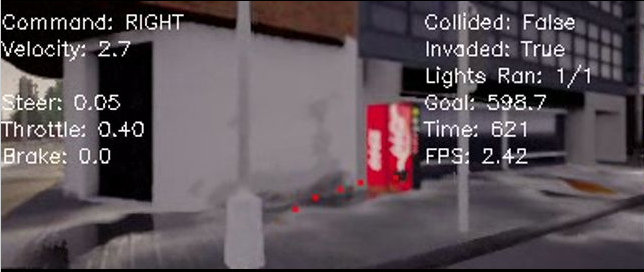
\includegraphics[width=6cm]{FOOL1.png}
    \label{fig:fool1}}
    \qquad
    \begin{minipage}{6cm}
    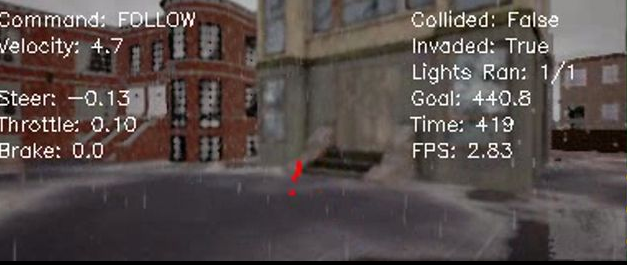
\includegraphics[width=6cm]{FOOL2.png}
    \label{fig:fool2}
    \end{minipage}
    \caption{Collisioni causate da NewtonFool.}
    \label{fig:foolrun}
    \end{figure}
\newpage
\subsection{Sintesi risultati}
I risultati raccolti (riassunti nella Tabella \ref{tab:ria}) confermano la vulnerabilità del modello considerato agli adversarial attacks. In tutti i casi l'affidabilità del veicolo si è ridotta.
L'attacco che ha causato problemi più gravi è sicuramente Basic Iterative Method. Mentre nelle altre run la traiettoria prestabilita continua ad essere quantomeno seguita, in questo
caso la macchina cambia completamente comportamento, diventando inutilizzabile.
\begin{table}[h]
    \begin{tabular}{|p{1.5cm}|p{2.5cm}|p{2cm}|p{1.5cm}|c|c|}
        \hline
        Attacco        &   Run completate     &   stabilità     &  semafori ignorati        & collisioni & timeout\\
        \hline
        Nessuno        &  12/12               &   ottima        &  0                       & 0          & 0 \\
        HSJ            &  6/12                &   bassa         &  9                        & 6          & 0 \\
        STA            &  7/12                &   discreta      &  0                        & 4          & 1 \\
        BIM            &  0/12                &   nulla         &  N/D                      & 12         & 0\\
        NF             &  3/12                &   bassa         &   13                      & 9          & 0 \\
        \hline
    \end{tabular}
    \caption{Riassunto dei risultati.}
    \label{tab:ria}
\end{table}